\newpage

\titleformat % design des titres des chapitres
{\chapter}
[display]
{\centering\normalfont\Large\scshape\bfseries}
{\rule[3pt]{0.15\linewidth}{3pt}\quad\chaptertitlename~\thechapter\quad \rule[3pt] {0.15\linewidth}{3pt}}
{0\baselineskip}%espace vertical entre chapitre et nom du chapitre
{\rule{\linewidth}{0.5pt}\break\Huge}
[\vspace{-0.5\baselineskip}\rule{\linewidth}{0.5pt}\vspace{0\baselineskip}]

\let\clearpage\relax% Stop LaTeX from going to a new page; and
\vspace*{5.5cm}%

\chapter{Etude Technique}
Dans ce chapitre, je vais présenter les outils de développement adoptés ainsi que
l’architecture technique et applicative du projet

\newpage

\section{Architecture Logique }

\begin{figure}[!h]
    \hspace{-1.1cm}
    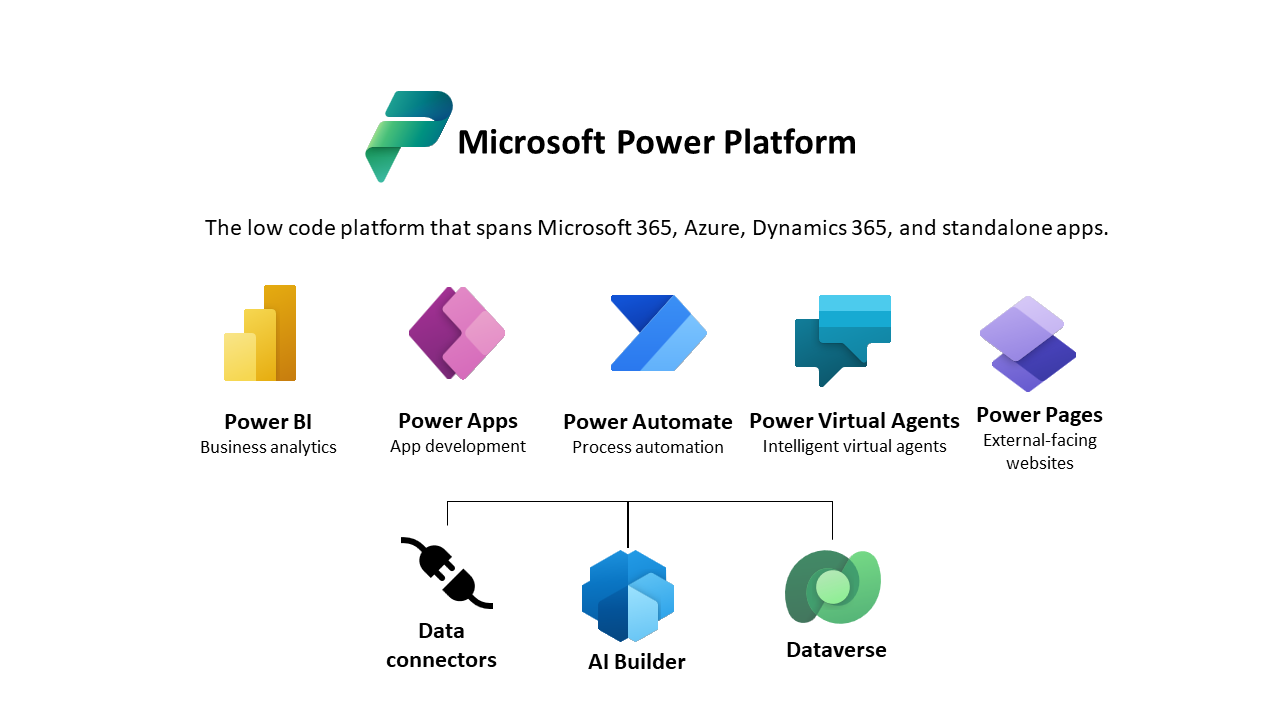
\includegraphics[scale=0.55,keepaspectratio]{Rapport de stage PFE chez DXC/figures/power platform.png}
    \caption{La suite Power Platform}
\end{figure}


Pour le développement de la solution nous avons utilisé Microsoft Power Platform qui permet la réalisation d'application web/mobile en low-code voire no-code. 
\\
\\
Le choix de ce dernier n'est pas anodin, en effet comme dit précédemment le projet souffrait de difficulté pour le verrouillage des exigences, notre client changeais d’avis tout le temps et il fallait pouvoir suivre ce changement, l’utilisation de technologie web très stricte aurait compliqué la tâche, tandis que l’environnement power platform nous a donné une sorte de flexibilité et a permis de toujours corriger ainsi que modifier les fonctionnalités selon le besoin du client dans des délais records.
\\



Les principaux composant de microsoft power platform sont:
\\

\begin{itemize}
  \item Power Apps 
  \item Power BI 
  \item Power Automate
  \item Power Virtual Agents
  \item Power Pages
\end{itemize}




\section{Architecture fonctionnelle}

Le projet Vallue Attainement consiste à mettre en place un système permettant un
échange entre différentes entités (RH, SL, Finance et Biz-DEV).
\\

L'architecture a été en pensé en trois version, l'architecture utilisée actuellement est proche de la premiere mais présentant d'abbord les differentes version.

\subsection{Architecture fonctionnelle - Version 1}

\begin{figure}[!h]
    \centering
    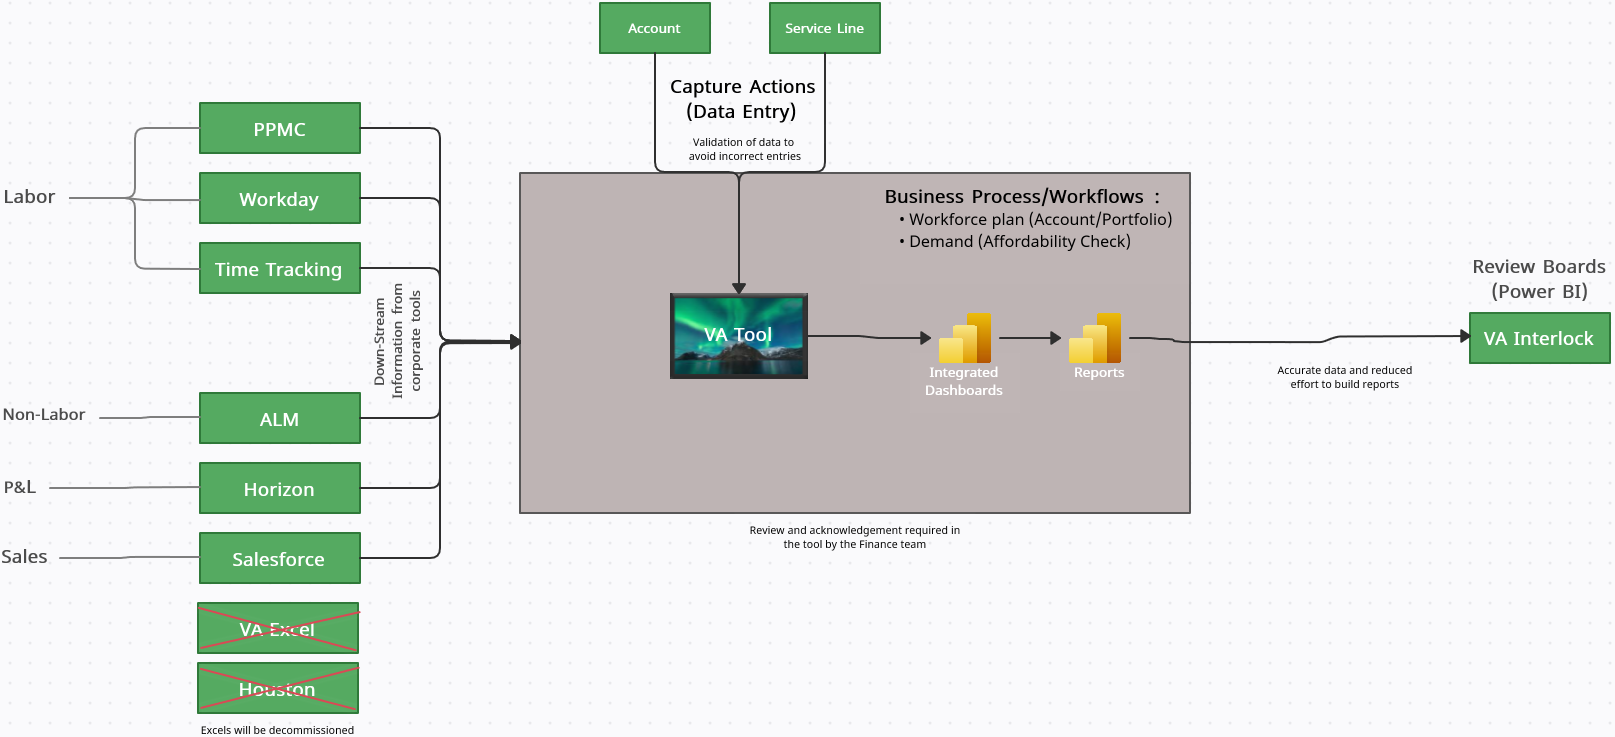
\includegraphics[scale=0.31,keepaspectratio]{Rapport de stage PFE chez DXC/figures/technical_model_version1.png}
    \caption{Architecture Fonctionnelle - Version 1}
\end{figure}

Donc on a une élimination des fichier Excel utilisée auparavant pour cette fois-ci offrir à l'utilisateur les données des différents outils DXC extraite de façon automatique mais aussi la main pour saisir les nouvelles données directement dans l'application pour les clients ainsi que les Service Lines et puis les stocker dans une base de données (Dataverse) et non un fichier Excel pour à la fin créer des tableaux de bord Power BI.


\newpage
\subsection{Architecture fonctionnelle - Version 2}
Dans la deuxieme version on va aussi relier la finance avec l'application pour permettre le traitement de cette derniere dans le meme outils comme montré dans la figure suivante:

\begin{figure}[!h]
    \centering
    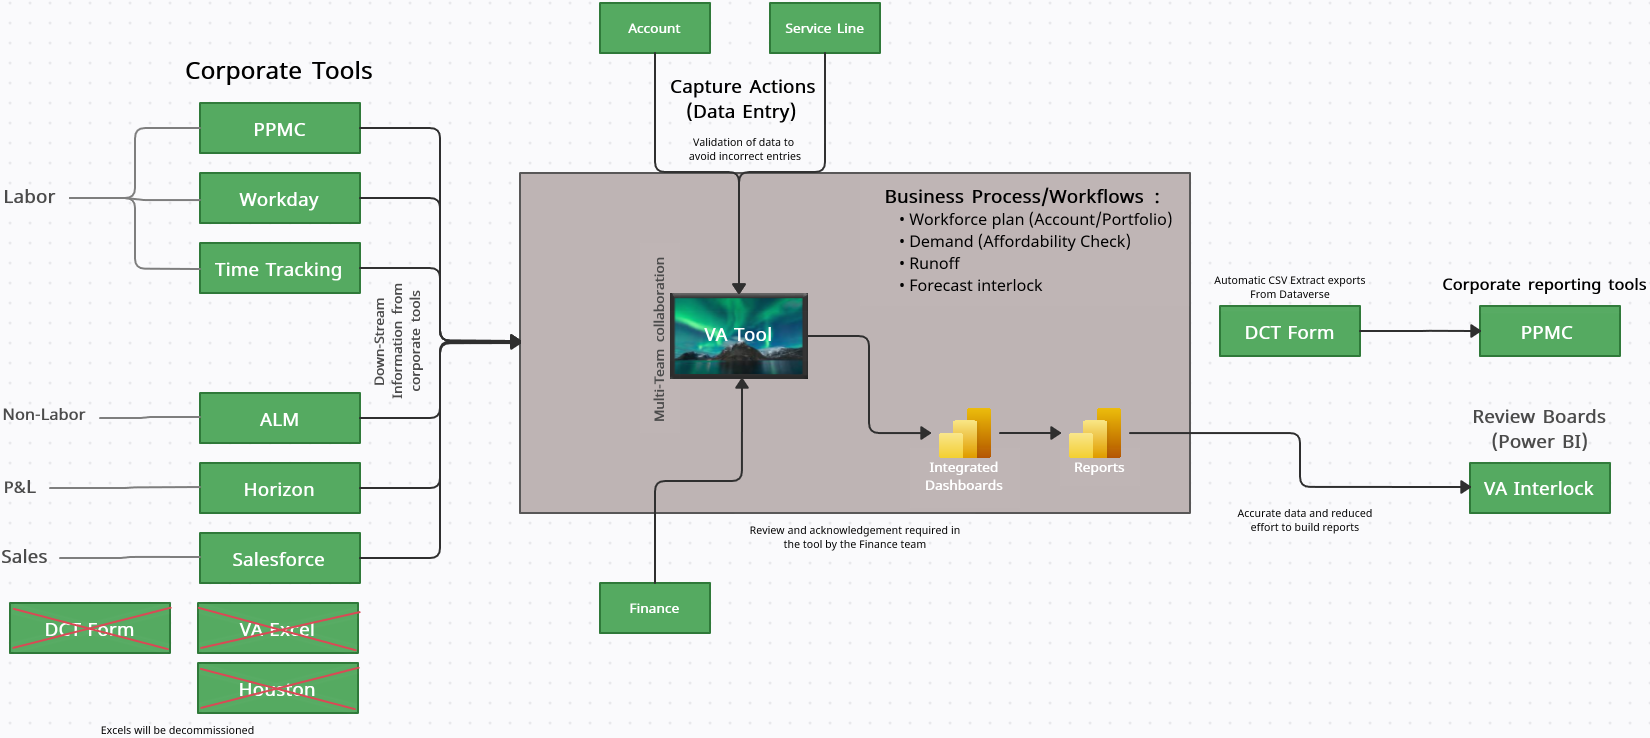
\includegraphics[scale=0.31,keepaspectratio]{Rapport de stage PFE chez DXC/figures/technical_model_version2.png}
    \caption{Architecture Fonctionnelle - Version 2}
\end{figure}

Donc encore une fois l'élimination des fichier Excel, mais aussi une liaison entre la finance et les différents clients ainsi que les services lines, on va aussi ajouter une extraction automatique du DCT form qui va être ensuite envoyé au PPMC un outil interne de DXC pour saisir cette information et prendre la decision.

\newpage
\subsection{Architecture fonctionnelle - Version 3}
La troisieme et finale version est une liaison entre tout les acteurs du systeme cette derniere va venir ajouter l'acteur RH a notre solution comme le montre la figure suivante:

\begin{figure}[!h]
    \centering
    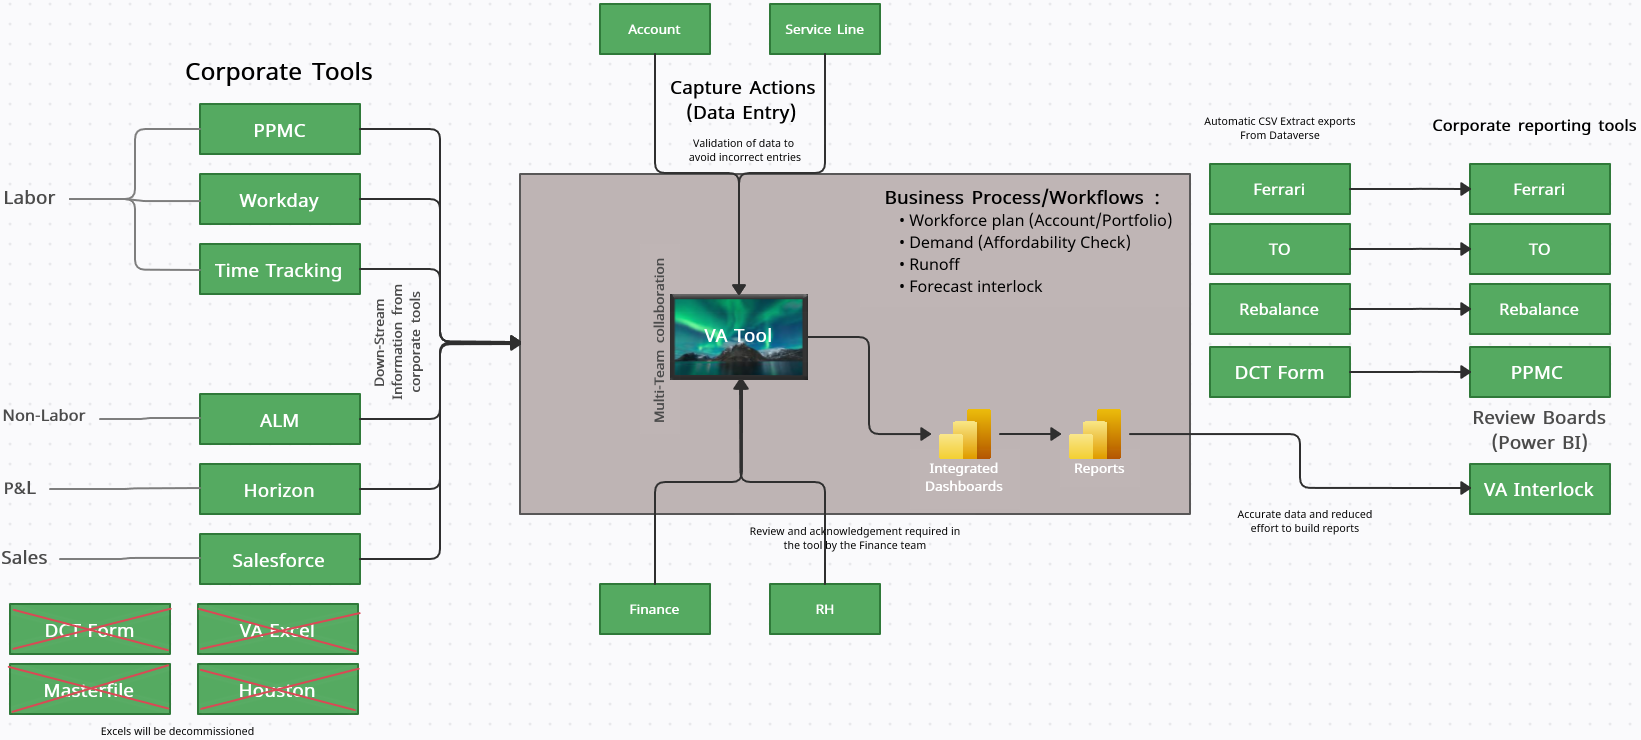
\includegraphics[scale=0.30,keepaspectratio]{Rapport de stage PFE chez DXC/figures/technical_model_version3.png}
    \caption{Architecture Fonctionnelle - Version 3}
\end{figure}

La version finale relie toutes les entités du système, elle va permettre une multi-collaboration entre les différentes équipes, ce qui va accélérer notre pipe commerciale, améliorer la circulation de l'information au sein de l'entreprise, créer un de cohésion, permettre à l'entreprise de mieux gérer ces deals.

\newpage
\subsection{Architecture fonctionnelle - Actuelle}

La version actuelle est s'approche de la premiere version comme le montre la figure suivante:

\begin{figure}[!h]
    \centering
    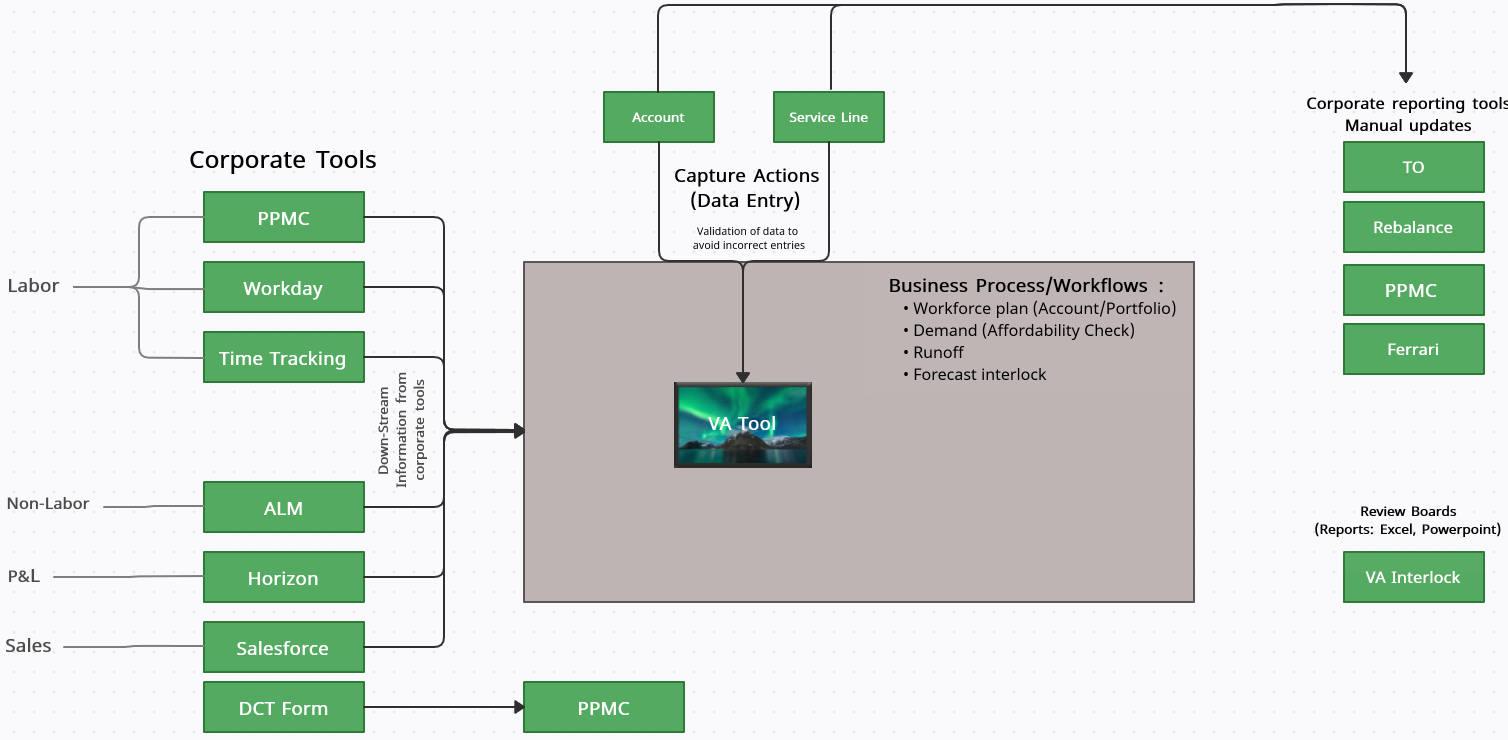
\includegraphics[scale=0.30,keepaspectratio]{Rapport de stage PFE chez DXC/figures/technical_model_version_actual.png}
    \caption{Architecture Fonctionnelle - actuelle}
\end{figure}

Comme le montre la figure suivante,les modifications ainsi que l'ajout des informations se fait d'une façon semi-automatique (utilisation de flow pour quelque informations) et les review boards se font toujours d'une manière classique à l'aide de fichier Excel et power point, cela revient à la difficulté de mettre les différents collaborateurs en accord.

\newpage
\section{Modèle de données}

La figure suivante represente l'architecture utilisée pour l'importation de la données: 
\begin{figure}[!h]
    \centering
    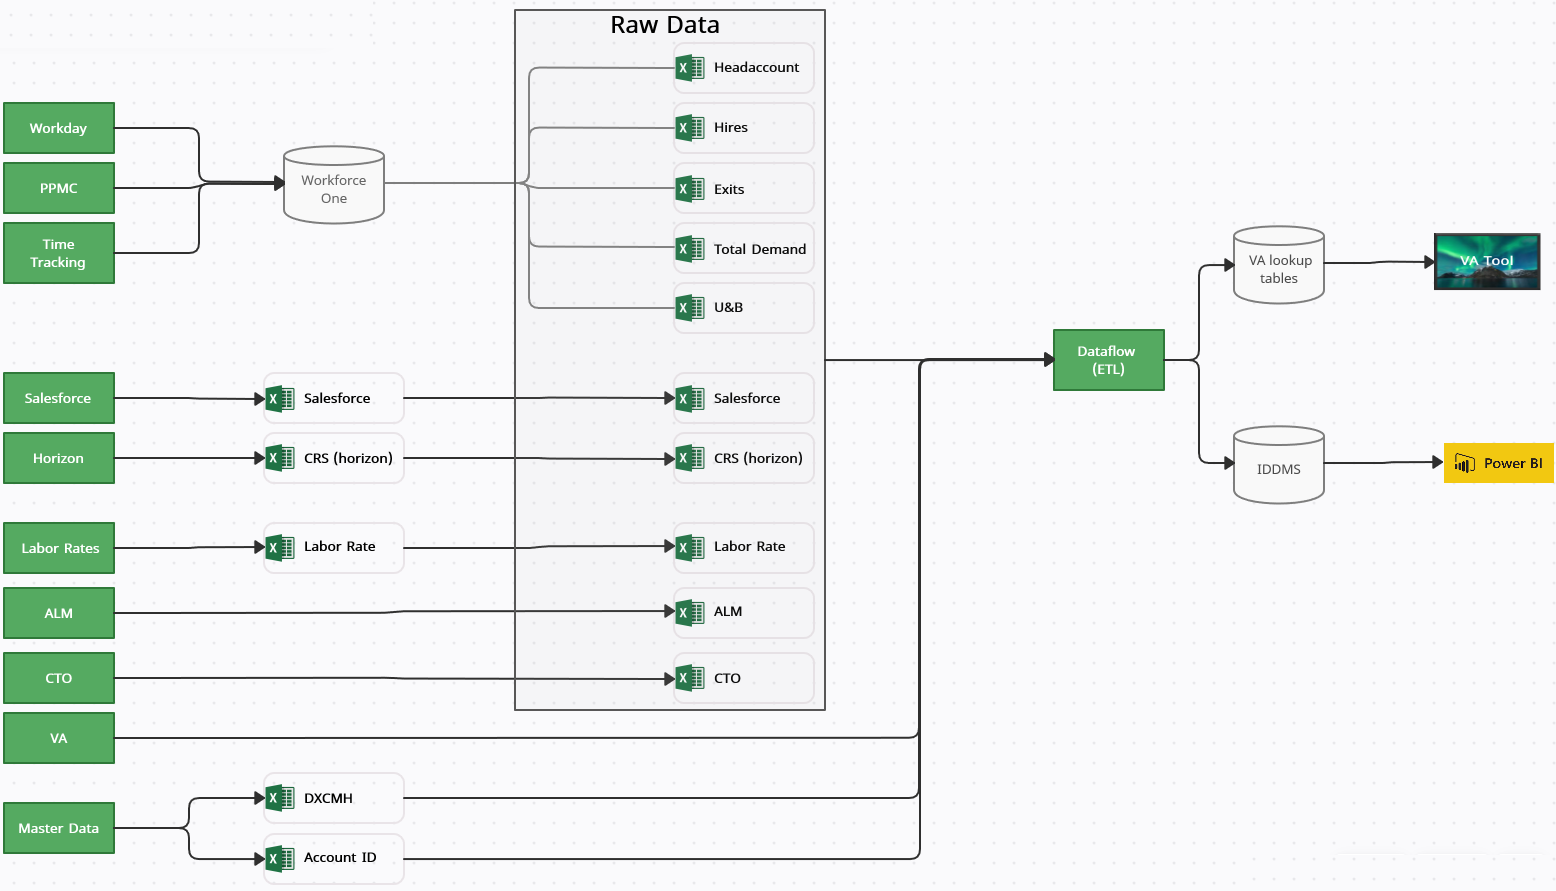
\includegraphics[scale=0.4,keepaspectratio]{Rapport de stage PFE chez DXC/figures/data_model.png}
    \caption{modèle de données}
\end{figure}

Pour l'importation de la donnée on peut voir l'existence de plusieurs fichier Excel l'avantage est que ces derniers pour la plupart sont générer automatiquement de la part des outils interne de l'entreprise, ce qui permet de rapidement les regrouper avec un seul Dataflow effectuer les différents changements (ETL) et les utilisé dans notre application ou bien pour créer des tableaux de bords.

\section{Architecture logiciel : Power Platform }

\subsection{Power Apps }
\vspace{0.5cm}

\begin{wrapfigure}{l}{0.4\textwidth}
  \begin{center}
    
\includegraphics[width=0.4\textwidth]{Rapport de stage PFE chez DXC/figures/power_apps.png}
  \end{center}
\end{wrapfigure}

Power Apps est une suite d’applications, de services, de connecteurs et une plateforme de données qui fournissent un environnement de développement rapide dans le but de concevoir des applications personnalisées et adaptées à vos besoins métier.
\\
\\
Les applications créées à l’aide de Power Apps fournissent une logique métier et des capacités de flux de travail enrichies pour transformer vos opérations d’entreprise manuels en processus numériques et automatisés. De plus, les applications conçues à l’aide de Power Apps ont une conception réactive et elles peuvent fonctionner de manière transparente dans un navigateur ou sur des appareils mobiles (téléphone ou tablette).


\subsection{Power Automate }

\begin{wrapfigure}{l}{0.4\textwidth}
  \begin{center}
    
\includegraphics[width=0.4\textwidth]{Rapport de stage PFE chez DXC/figures/power_automate.png}
  \end{center}
\end{wrapfigure}

Power automate est un puissant outils d'automatisation qui permet de :
\begin{itemize}
  \item Automatiser les processus d’entreprise
  \item envoyer des rappels automatiques sur les tâches en retard ;
  \item Se connecter à plus de 500 sources de données ou à toute API accessible au public
\end{itemize}
\\ 
\\
Tout cela sans avoir conaissance technique specifique, n'importe quelle utilisateur pourrait créer ainsi que manipuler des processus automatisée en utilisant la plateforme Power Automate qui represente elle aussi un environement low-code/no-code

\subsection{Power BI }

\begin{wrapfigure}{l}{0.4\textwidth}
  \begin{center}
    
\includegraphics[width=0.4\textwidth]{Rapport de stage PFE chez DXC/figures/power_bi.png}
  \end{center}
\end{wrapfigure}

Power BI est un ensemble de services logiciels, d’applications et de connecteurs qui œuvrent ensemble pour transformer des sources de données disparates en informations visuelles immersives et interactives. 
\\
Vos données peuvent être sous forme de feuille de calcul Excel ou de collection d’entrepôts de données hybrides locaux ou sur le cloud. Power BI vous permet de vous connecter facilement à vos sources de données, de visualiser et de découvrir ce qui est important.

\subsection{Power virtual agent }

\begin{wrapfigure}{l}{0.4\textwidth}
  \begin{center}
    
\includegraphics[width=0.4\textwidth]{Rapport de stage PFE chez DXC/figures/power_virtual_agent.png}
  \end{center}
\end{wrapfigure}

Power Virtual Agents vous permet de créer des chatbots puissants qui peuvent répondre aux questions posées par vos clients, d’autres employés ou des visiteurs de votre site Web ou service.

Ces bots peuvent être créés facilement sans avoir besoin de spécialistes des données ou de développeurs.

Power Virtual Agents est disponible à la fois en tant qu’application Web autonome et en tant qu’application distincte dans Microsoft Teams.

\subsection{Power Pages}

\begin{wrapfigure}{l}{0.4\textwidth}
  \begin{center}
    
\includegraphics[width=0.22\textwidth]{Rapport de stage PFE chez DXC/figures/power_pages_logo.JPG}
  \end{center}
\end{wrapfigure}

Microsoft Power Pages est une plate-forme logicielle en tant que service (SaaS) sécurisée,à faible code pour la création, destinés a l'hébergement et l'administration de sites Web d'entreprise modernes à l'extérieur. 
\\\\
Que vous soyez un créateur low-code ou un développeur professionnel, Power Pages vous permet de concevoir, configurer et publier rapidement des sites Web qui fonctionnent de manière transparente sur tous les navigateurs et appareils Web.
\\\\
Power Pages vous offre des modèles riches et personnalisables, une expérience visuelle fluide grâce à un studio de conception repensé et un nouveau centre d'apprentissage intégré pour créer rapidement des sites qui répondent aux besoins uniques de votre entreprise.

\subsection{Dataverse }

\begin{wrapfigure}{l}{0.35\textwidth}
  \begin{center}
    
\includegraphics[width=0.24\textwidth]{Rapport de stage PFE chez DXC/figures/dataverse.png}
  \end{center}
\end{wrapfigure}

Dataverse permet de stocker et de gérer en toute sécurité les données utilisées par les applications métier. Les données à l’intérieur de Dataverse sont stockées dans un ensemble de tables. Une table est un ensemble de lignes (anciennement appelées enregistrements) et de colonnes (anciennement appelées champs / attributs). 
\\\\
Chaque colonne de la tables est conçue pour stocker un certain type de données, par exemple, le nom, l’âge, le salaire, etc. 
\\\\
Dataverse comprend un ensemble de base de tables standard qui couvrent des scénarios classiques, mais vous pouvez également créer des tables personnalisées dédiées à votre organisation et les remplir avec des données à l’aide de Power Query. 

\section{Conclusion}
Dans ce chapitre j'ai montré les différentes versions de l'architecture fonctionnelle de l'application ainsi qu'une petite description de Power Platform, le chapitre suivant va nous montrer la réalisation de l'application et les différents pages créer.




